\chapter{ಲೇಖನಿ – ಚಿತ್ರ ಬಿಡಿಸುವುದು}

\section{ಲೇಖನಿಯುಕ್ತ - ಮುಕ್ತ}
\begin{figure}[h]
\begin{center}
\begin{multicols}{2}
\begin{Scratch}[1]
\beginbox{}
\scbox{ಲೇಖನಿಯುಕ್ತ}{pen}
\scbox{\cb[w]{100} ಹೆಜ್ಜೆ ಮುಂದೆ ಹೋಗು}{motion}
\turnbox{1}{90}{ಡಿಗ್ರಿಯಷ್ಟು ತಿರುಗು}
\scbox{\cb[w]{100} ಹೆಜ್ಜೆ ಮುಂದೆ ಹೋಗು}{motion}
\turnbox{1}{90}{ಡಿಗ್ರಿಯಷ್ಟು ತಿರುಗು}
\scbox{\cb[w]{100} ಹೆಜ್ಜೆ ಮುಂದೆ ಹೋಗು}{motion}
\turnbox{1}{90}{ಡಿಗ್ರಿಯಷ್ಟು ತಿರುಗು}
\scbox{\cb[w]{100} ಹೆಜ್ಜೆ ಮುಂದೆ ಹೋಗು}{motion}
\end{Scratch}

\begin{tikzpicture}
\node[doc] (x) (inst1){
ಒತ್ತಿದಾಗ\\
ಲೇಖನಿಯುಕ್ತ\\
100  ಹೆಜ್ಜೆ ಮುಂದೆ ಹೋಗು\\
90$‌^\circ$ ಬಲಕ್ಕೆ  ತಿರುಗು\\
100  ಹೆಜ್ಜೆ ಮುಂದೆ ಹೋಗು\\
90$‌^\circ$ ಬಲಕ್ಕೆ  ತಿರುಗು\\
100  ಹೆಜ್ಜೆ ಮುಂದೆ ಹೋಗು\\
90$‌^\circ$ ಬಲಕ್ಕೆ  ತಿರುಗು\\
100  ಹೆಜ್ಜೆ ಮುಂದೆ ಹೋಗು
};
\end{tikzpicture}

\end{multicols}

\begin{tikzpicture}
\node at (0,0)[rotate=0, opacity=0.2](s1){};
\draw[draw=blue](s1.center)--++(2cm,0)node(newcoord){};
\node at (newcoord)[rotate=-90, opacity=0.2](s2){};
\draw[draw=blue](s2.center)--++(0,-2cm)node(newcoord){};
\node at (newcoord)[rotate=-180, opacity=0.2](s3){};
\draw[draw=blue](s3.center)--++(-2cm,0cm)node(newcoord){};
\node at (newcoord)[rotate=90, opacity=0.2](s4){};
\draw[draw=blue](s4.center)--++(0,2cm)node(newcoord){};
\node at (newcoord)[rotate=90, opacity=1](s2){\Scratchy[0.2]};
\end{tikzpicture}
\end{center}
\caption{ಸ್ಪ್ರಯ್ಟ್  ಚೌಕ ಬಿಡಿಸುವುದು}
\label{sqr}
\end{figure}

\begin{figure}[h]
\begin{center}
\begin{multicols}{2}
\begin{Scratch}[1]
\beginbox{}
\scbox{ಲೇಖನಿಯುಕ್ತ}{pen}
\scbox{\cb[w]{100} ಹೆಜ್ಜೆ ಮುಂದೆ ಹೋಗು}{motion}
\scbox{ಲೇಖನಿಮುಕ್ತ}{pen}
\scbox{\cb[w]{100} ಹೆಜ್ಜೆ ಮುಂದೆ ಹೋಗು}{motion}
\scbox{ಲೇಖನಿಯುಕ್ತ}{pen}
\scbox{\cb[w]{100} ಹೆಜ್ಜೆ ಮುಂದೆ ಹೋಗು}{motion}
\end{Scratch}

\begin{tikzpicture}
\node[doc] (x) (inst1){
ಒತ್ತಿದಾಗ\\
ಲೇಖನಿಯುಕ್ತ\\
100  ಹೆಜ್ಜೆ ಮುಂದೆ ಹೋಗು\\
ಲೇಖನಿಮುಕ್ತ\\
100  ಹೆಜ್ಜೆ ಮುಂದೆ ಹೋಗು\\
ಲೇಖನಿಯುಕ್ತ\\
100  ಹೆಜ್ಜೆ ಮುಂದೆ ಹೋಗು
};
\end{tikzpicture}

\end{multicols}

\begin{tikzpicture}
\node at (0,0)[rotate=0, opacity=0.2](s1){};
\draw[draw=blue](s1.center)--++(2cm,0)node(newcoord){};
\node at (newcoord)[rotate=0, opacity=0.2](s2){};
\draw[draw=none](s2.center)--++(2cm,0cm)node(newcoord){};
\node at (newcoord)[rotate=-0, opacity=0.2](s3){};
\draw[draw=blue](s3.center)--++(2cm,0cm)node(newcoord){};
\node at (newcoord)[rotate=0, opacity=1](s4){\Scratchy[0.2]};
\end{tikzpicture}
\end{center}
\caption{ಸ್ಪ್ರಯ್ಟ್ ಇಂದ್ ಮುರಿದ ರೇಖೆ ಬಿಡಿಸುವುದು}
\label{sqr}
\end{figure}

\section{ಗಾತ್ರ ಬದಲಾಯಿಸುವುದು}

\begin{figure}[h]
\begin{center}
\begin{multicols}{2}
\begin{Scratch}[1]
\beginbox{}
\scbox{ಲೇಖನಿಯುಕ್ತ}{pen}
\scbox{\cb[w]{100} ಹೆಜ್ಜೆ ಮುಂದೆ ಹೋಗು}{motion}
\scbox{\cb[w]{100} ಹೆಜ್ಜೆ ಮುಂದೆ ಹೋಗು}{pen}
\scbox{\cb[w]{100} ಹೆಜ್ಜೆ ಮುಂದೆ ಹೋಗು}{motion}
\scbox{\cb[w]{100} ಹೆಜ್ಜೆ ಮುಂದೆ ಹೋಗು}{pen}
\scbox{\cb[w]{100} ಹೆಜ್ಜೆ ಮುಂದೆ ಹೋಗು}{motion}
\end{Scratch}

\begin{tikzpicture}
\node[doc] (x) (inst1){
ಒತ್ತಿದಾಗ\\
ಲೇಖನಿಯುಕ್ತ\\
100  ಹೆಜ್ಜೆ ಮುಂದೆ ಹೋಗು\\
100  ಹೆಜ್ಜೆ ಮುಂದೆ ಹೋಗು\\
100  ಹೆಜ್ಜೆ ಮುಂದೆ ಹೋಗು
};
\end{tikzpicture}

\end{multicols}

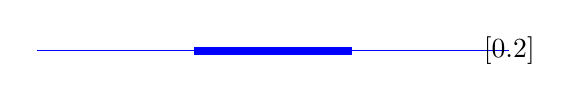
\begin{tikzpicture}
\node at (0,0)[rotate=0, opacity=0.2](s1){};
\draw[draw=blue](s1.center)--++(2cm,0)node(newcoord){};
\node at (newcoord)[rotate=0, opacity=0.2](s2){};
\draw[draw=blue, line width=3pt](s2.center)--++(2cm,0cm)node(newcoord){};
\node at (newcoord)[rotate=-0, opacity=0.2](s3){};
\draw[draw=blue](s3.center)--++(2cm,0cm)node(newcoord){};
\node at (newcoord)[rotate=0, opacity=1](s4){\Scratchy[0.2]};
\end{tikzpicture}
\end{center}
\caption{ಲೇಖನಿ ಗಾತ್ರ ಬದಲಾಯಿಸುವುದು}
\label{sqr}
\end{figure}

\begin{figure}[h]
\begin{center}
\begin{multicols}{2}
\begin{Scratch}[1]
\beginbox{}
\scbox{ಲೇಖನಿಯುಕ್ತ}{pen}
\scbox{\cb[w]{100} ಹೆಜ್ಜೆ ಮುಂದೆ ಹೋಗು}{motion}
\scbox{\cb[w]{100} ಹೆಜ್ಜೆ ಮುಂದೆ ಹೋಗು}{pen}
\scbox{\cb[w]{100} ಹೆಜ್ಜೆ ಮುಂದೆ ಹೋಗು}{motion}
\scbox{\cb[w]{100} ಹೆಜ್ಜೆ ಮುಂದೆ ಹೋಗು}{pen}
\scbox{\cb[w]{100} ಹೆಜ್ಜೆ ಮುಂದೆ ಹೋಗು}{motion}
\end{Scratch}

\begin{tikzpicture}
\node[doc] (x) (inst1){
ಒತ್ತಿದಾಗ\\
ಲೇಖನಿಯುಕ್ತ\\
100  ಹೆಜ್ಜೆ ಮುಂದೆ ಹೋಗು\\
ಲೇಖನಿಮುಕ್ತ\\
100  ಹೆಜ್ಜೆ ಮುಂದೆ ಹೋಗು\\
ಲೇಖನಿಯುಕ್ತ\\
100  ಹೆಜ್ಜೆ ಮುಂದೆ ಹೋಗು
};
\end{tikzpicture}

\end{multicols}

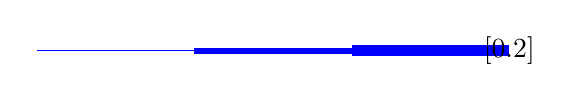
\begin{tikzpicture}
\node at (0,0)[rotate=0, opacity=0.2](s1){};
\draw[draw=blue](s1.center)--++(2cm,0)node(newcoord){};
\node at (newcoord)[rotate=0, opacity=0.2](s2){};
\draw[draw=blue, line width=2pt](s2.center)--++(2cm,0cm)node(newcoord){};
\node at (newcoord)[rotate=-0, opacity=0.2](s3){};
\draw[draw=blue, line width=4pt](s3.center)--++(2cm,0cm)node(newcoord){};
\node at (newcoord)[rotate=0, opacity=1](s4){\Scratchy[0.2]};
\end{tikzpicture}
\end{center}
\caption{ಲೇಖನಿ ಗಾತ್ರವನ್ನು ಸಾಪೇಕ್ಷವಾಗಿ ಬದಲಾಯಿಸುವುದು}
\label{pensize}
\end{figure}

\section{ಬಣ್ಣ ಬದಲಾಯಿಸುವುದು}

\begin{figure}[h]
\begin{center}
\begin{multicols}{2}
\begin{Scratch}[1]
\beginbox{}
\scbox{ಲೇಖನಿಯುಕ್ತ}{pen}
\scbox{\cb[w]{100} ಹೆಜ್ಜೆ ಮುಂದೆ ಹೋಗು}{motion}
\scbox{\cb[w]{100} ಹೆಜ್ಜೆ ಮುಂದೆ ಹೋಗು}{pen}
\scbox{\cb[w]{100} ಹೆಜ್ಜೆ ಮುಂದೆ ಹೋಗು}{motion}
\scbox{\cb[w]{100} ಹೆಜ್ಜೆ ಮುಂದೆ ಹೋಗು}{pen}
\scbox{\cb[w]{100} ಹೆಜ್ಜೆ ಮುಂದೆ ಹೋಗು}{motion}
\end{Scratch}

\begin{tikzpicture}
\node[doc] (x) (inst1){
ಒತ್ತಿದಾಗ\\
ಲೇಖನಿಯುಕ್ತ\\
100  ಹೆಜ್ಜೆ ಮುಂದೆ ಹೋಗು\\
100  ಹೆಜ್ಜೆ ಮುಂದೆ ಹೋಗು\\
100  ಹೆಜ್ಜೆ ಮುಂದೆ ಹೋಗು
};
\end{tikzpicture}

\end{multicols}

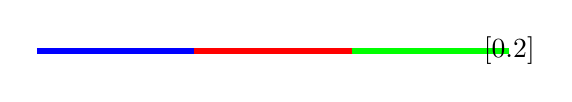
\begin{tikzpicture}
\node at (0,0)[rotate=0, opacity=0.2](s1){};
\draw[draw=blue,line width=2pt](s1.center)--++(2cm,0)node(newcoord){};
\node at (newcoord)[rotate=0, opacity=0.2](s2){};
\draw[draw=red, line width=2pt](s2.center)--++(2cm,0cm)node(newcoord){};
\node at (newcoord)[rotate=-0, opacity=0.2](s3){};
\draw[draw=green,line width=2pt](s3.center)--++(2cm,0cm)node(newcoord){};
\node at (newcoord)[rotate=0, opacity=1](s4){\Scratchy[0.2]};
\end{tikzpicture}
\end{center}
\caption{ಲೇಖನಿ ಬಣ್ಣ ಬದಲಾಯಿಸುವುದು}
\label{sqr}
\end{figure}

\begin{figure}[h]
\begin{center}
\begin{multicols}{2}
\begin{Scratch}[1]
\beginbox{}
\scbox{ಲೇಖನಿಯುಕ್ತ}{pen}
\scbox{\cb[w]{100} ಹೆಜ್ಜೆ ಮುಂದೆ ಹೋಗು}{motion}
\scbox{\cb[w]{100} ಹೆಜ್ಜೆ ಮುಂದೆ ಹೋಗು}{pen}
\scbox{\cb[w]{100} ಹೆಜ್ಜೆ ಮುಂದೆ ಹೋಗು}{motion}
\scbox{\cb[w]{100} ಹೆಜ್ಜೆ ಮುಂದೆ ಹೋಗು}{pen}
\scbox{\cb[w]{100} ಹೆಜ್ಜೆ ಮುಂದೆ ಹೋಗು}{motion}
\end{Scratch}

\begin{tikzpicture}
\node[doc] (x) (inst1){
ಒತ್ತಿದಾಗ\\
ಲೇಖನಿಯುಕ್ತ\\
100  ಹೆಜ್ಜೆ ಮುಂದೆ ಹೋಗು\\
ಲೇಖನಿಮುಕ್ತ\\
100  ಹೆಜ್ಜೆ ಮುಂದೆ ಹೋಗು\\
ಲೇಖನಿಯುಕ್ತ\\
100  ಹೆಜ್ಜೆ ಮುಂದೆ ಹೋಗು
};
\end{tikzpicture}

\end{multicols}

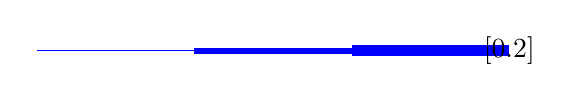
\begin{tikzpicture}
\node at (0,0)[rotate=0, opacity=0.2](s1){};
\draw[draw=blue](s1.center)--++(2cm,0)node(newcoord){};
\node at (newcoord)[rotate=0, opacity=0.2](s2){};
\draw[draw=blue, line width=2pt](s2.center)--++(2cm,0cm)node(newcoord){};
\node at (newcoord)[rotate=-0, opacity=0.2](s3){};
\draw[draw=blue, line width=4pt](s3.center)--++(2cm,0cm)node(newcoord){};
\node at (newcoord)[rotate=0, opacity=1](s4){\Scratchy[0.2]};
\end{tikzpicture}
\end{center}
\caption{ಲೇಖನಿ ಬಣ್ಣವನ್ನು ಸಾಪೇಕ್ಷವಾಗಿ ಬದಲಾಯಿಸುವುದು}
\label{sqr}
\end{figure}


\section{ಅಭ್ಯಾಸ }
\begin{enumerate}
\item{ಸ್ಪ್ರಯ್ಟ್ ಆಯತವನ್ನು ಬಿಡಿಸುವಂತೆ ಪ್ರೊಗ್ರಾಂ ಬರೆಯಿರಿ. ಮೊದಲು ಪುಸ್ತಕದಲ್ಲಿ ಪ್ರಯತ್ನಿಸಿ ನಂತರ ಸ್ಕ್ರಾಚ್ನಲ್ಲಿ ಮಾಡಿ ನೋಡಿ. }


\begin{figure}[h]
\begin{center}
\begin{tikzpicture}
\node at (0,0)[draw=blue,  rectangle, minimum width = 4cm, minimum height=2cm](s1){};
\node at (s1.north east)[rotate=0, opacity=1](s2){\Scratchy[0.2]};
\end{tikzpicture}
\end{center}
\caption{ಸ್ಪ್ರಯ್ಟ್ ಇಂದ  ಆಯತವನ್ನು ಬಿಡಿಸುವುದು}
\label{pen_program1}
\end{figure}

\item{ಸ್ಪ್ರಯ್ಟ್ ಕೇಂದ್ರೀಕೃತ ಚೌಕವನ್ನು ಬಿಡಿಸುವಂತೆ ಪ್ರೊಗ್ರಾಂ ಬರೆಯಿರಿ. ಮೊದಲು ಪುಸ್ತಕದಲ್ಲಿ ಪ್ರಯತ್ನಿಸಿ ನಂತರ ಸ್ಕ್ರಾಚ್ನಲ್ಲಿ ಮಾಡಿ ನೋಡಿ. }


\begin{figure}[h]
\begin{center}

\begin{tikzpicture}
\node at (0,0)[draw=blue,  rectangle, minimum width = 4cm, minimum height=4cm](s1){};
\node at (s1.north east)[rotate=0, opacity=1](s2){\Scratchy[0.2]};
\node at (s1.center)[anchor=center, draw=blue,  rectangle, minimum width = 2cm, minimum height=2cm](s3){};
\end{tikzpicture}
\end{center}
\caption{ಸ್ಪ್ರಯ್ಟ್ ಇಂದ ಕೇಂದ್ರೀಕೃತ ಚೌಕವನ್ನು ಬಿಡಿಸುವುದು}
\label{pen_program2}
\end{figure}

\item{ಸ್ಪ್ರಯ್ಟ್ ಇಂದ ಮುರಿದ ರೇಖೆಗಳ ಚೌಕವನ್ನು ಬಿಡಿಸುವಂತೆ ಪ್ರೊಗ್ರಾಂ ಬರೆಯಿರಿ. }


\begin{figure}[h]
\begin{center}
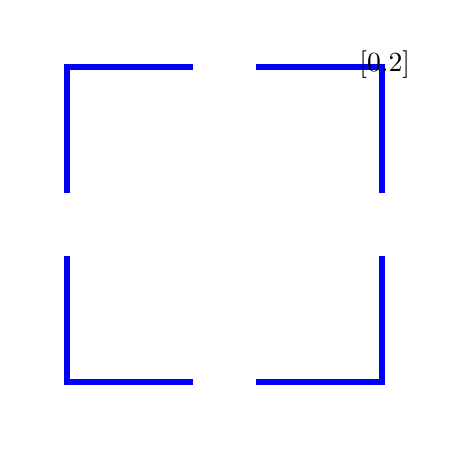
\begin{tikzpicture}
\node at (0,0)[draw=blue,  line width = 2pt, rectangle, minimum width = 4cm, minimum height=4cm](s1){};
\node at (s1.center)[anchor=center, draw=none,  fill=white, rectangle, minimum width = 0.8cm, minimum height=5cm](s2){};
\node at (s1.center)[anchor=center, draw=none,  fill=white, rectangle, minimum width = 5cm, minimum height=0.8cm](s3){};
\node at (s1.north east)[rotate=0, opacity=1](s4){\Scratchy[0.2]};
\end{tikzpicture}
\end{center}
\caption{ಸ್ಪ್ರಯ್ಟ್ ಇಂದ ಮುರಿದ-ರೇಖೆಗಳ ಚೌಕವನ್ನು ಬಿಡಿಸುವುದು}
\label{pen_program3}
\end{figure}

\item{ಸ್ಪ್ರಯ್ಟ್ ಇಂದ ವಿವಿಧ ಗಾತ್ರದ ರೇಖೆಗಳ ಚೌಕವನ್ನು ಬಿಡಿಸುವಂತೆ ಪ್ರೊಗ್ರಾಂ ಬರೆಯಿರಿ. }

\begin{figure}[h]
\begin{center}
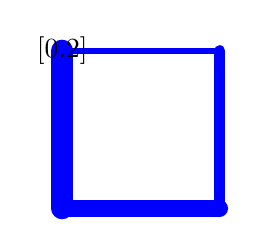
\begin{tikzpicture}
\draw[draw=blue, line width=2pt,line cap=round] (0,0)--++(2cm,0) coordinate (a);
\draw[draw=blue, line width=4pt,line cap=round] (a)--++(0,-2cm) coordinate (a);
\draw[draw=blue, line width=6pt,line cap=round] (a)--++(-2cm,0) coordinate (a);
\draw[draw=blue, line width=8pt,line cap=round] (a)--++(0,2cm) coordinate (a);
\node at (a)[rotate=0, opacity=1, anchor=center](s4){\Scratchy[0.2]};
\end{tikzpicture}
\end{center}
\caption{ಸ್ಪ್ರಯ್ಟ್ ಇಂದ ವಿವಿಧ ಗಾತ್ರದ ರೇಖೆಗಳಿಂದ ಚೌಕವನ್ನು ಬಿಡಿಸುವುದು}
\label{pen_program4}
\end{figure}

\item{ಸ್ಪ್ರಯ್ಟ್ ಇಂದ ವಿವಿಧ ಬಣ್ಣದ ರೇಖೆಗಳ ಚೌಕವನ್ನು ಬಿಡಿಸುವಂತೆ ಪ್ರೊಗ್ರಾಂ ಬರೆಯಿರಿ. }

\begin{figure}[h]
\begin{center}
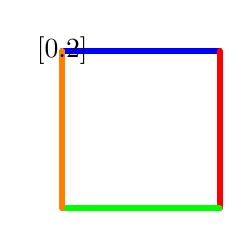
\begin{tikzpicture}
\draw[draw=blue, line width=2pt,line cap=round] (0,0)--++(2cm,0) coordinate (a);
\draw[draw=red, line width=2pt,line cap=round] (a)--++(0,-2cm) coordinate (a);
\draw[draw=green, line width=2pt,line cap=round] (a)--++(-2cm,0) coordinate (a);
\draw[draw=orange, line width=2pt,line cap=round] (a)--++(0,2cm) coordinate (a);
\node at (a)[rotate=0, opacity=1, anchor=center](s4){\Scratchy[0.2]};
\end{tikzpicture}
\end{center}
\caption{ಸ್ಪ್ರಯ್ಟ್ ಇಂದ ವಿವಿಧ ಬಣ್ಣದ ರೇಖೆಗಳಿಂದ ಚೌಕವನ್ನು ಬಿಡಿಸುವುದು}
\label{pen_program5}
\end{figure}

\end{enumerate}